\section{Описание предлагаемого подхода}
В этом разделе описывается предлагаемый подход к классификации функций.

\subsection{Алгоритм классификации функций в бинарном коде}
Программный комплекс, решающий задачу определения поведения функций, состоит из фреймворков McSema и NCC.

Предлагаемый алгоритм получения меток для каждой функции в бинарном исполняемом файле выглядит следующим образом: 
\begin{enumerate}
    \item На первом этапе исполняемый бинарный файл подается в программу mcsema-disas из фреймворка McSema, из него извлекается граф потока управления;
    \item Полученный на предыдущем шаге файл подается в программу mcsema-lift из фреймворка McSema, который переводит файл в llvm биткод;
    \item Файл с llvm биткодом переводится программой llvm-dis из фреймворка LLVM в представление llvm ir;
    \item Полученный файл подается на вход программы classifyapp. Программа выполняет следующие действия: 
    \begin{enumerate}
        \item Файл с llvm ir разбивается на функции, каждая функция сохраняется в отдельном файле;
        \item Все инструкции в файлах заменяются на их векторные представления (брались предобученные векторы из фреймворка NCC);
        \item Файлы поступают на вход рекуррентной нейронной сети, которая возвращает распределение вероятностей принадлежности функции классам;
        \item Из полученного распределения сохраняются в отдельный файл в json формате 3 меток классов с максимальными вероятностями.
    \end{enumerate}
    \item На последнем шаге с помощью плагина полученный json файл загружается в Ida Pro и для каждой функции создаётся комментарий с 3 полученными метками классов.
\end{enumerate}

Данный алгоритм изображён на рисунке \ref{ris:sugested_approach}.
\begin{figure}[h]
    \center{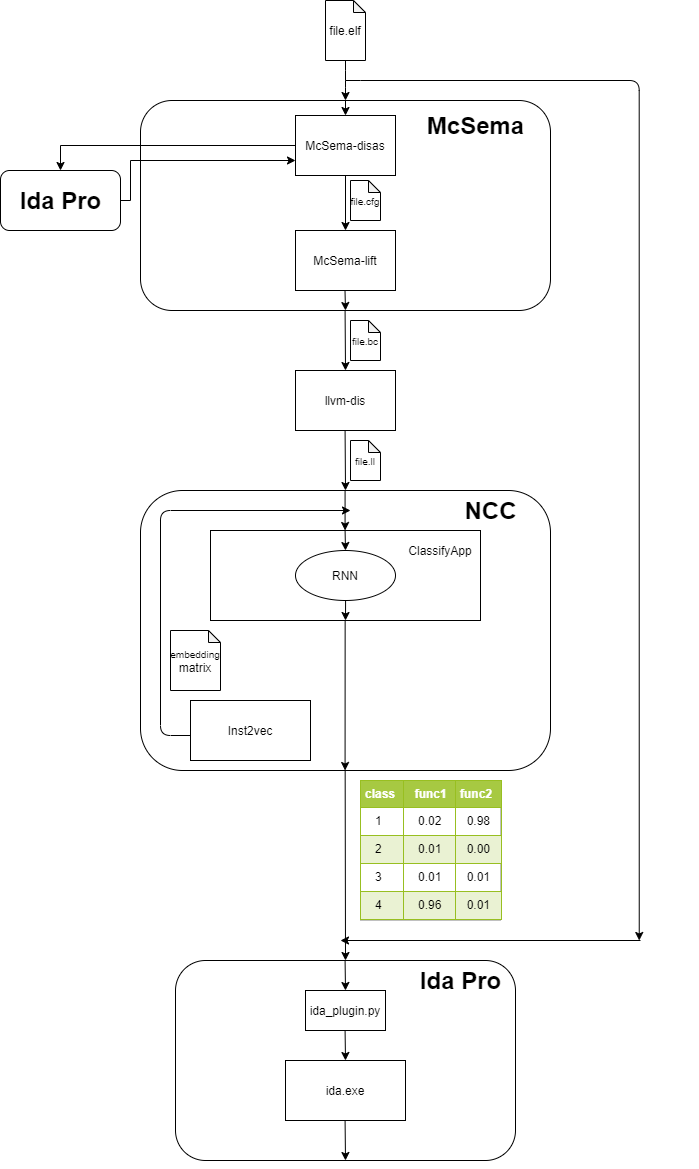
\includegraphics[width=0.70\linewidth,height=0.72\textheight]{images/scheme_vert.png}}
    \caption{Предлагаемый алгоритм классификации функций в бинарном файле}
    \label{ris:sugested_approach}
\end{figure}

\subsection{Обучение рекуррентной нейронной сети}
Рекуррентная нейронная сеть состояла из двух SRU\cite{lei2018simple} блоков, слоя нормализации LayerNorm\cite{LayerNorm} перед каждым SRU блоком, слоя Dropout между SRU блоками и полносвязного слоя. В модели было обучаемых параметров.

В качестве функции ошибки использовалась функция cross-entropy loss и метод оптимизации Adam.

Все последовательности дополнялись до 830 токенов или обрезались, если их длина была больше.

Перебор гиперпараметров производился с помощью алгоритма ASHA\cite{li2018massively}.

Код программной реализации находится в открытом доступе\footnote{\url{https://github.com/vladimirtelepov/ncc}}

\subsection{Результаты обучения рекуррентной нейронной сети}
Была получена доля верно угаданных меток $\%$ на тренировочной выборке, $\%$ на валидационной выборке и $\%$ на тестовой выборке, графики зависимостей от количества эпох можно увидеть на рисунках \ref{ris:loss} и \ref{ris:acc}. На обоих рисунках синяя линия соответствует тренировочной выборке, желтая - валидационной.

\subsection{Ограничения подхода}
Из предыдущей секции можно сделать вывод о том, что предложенный подход применим для анализа больших бинарных программ и сложных алгоритмов. Однако у данного подхода есть следующие ограничения:
\begin{enumerate}
    \item Mcsema не всегда может перевести в llvm ir бинарный файл, и результат ее работы сильно зависит от дизассемблера. Также нужно учесть, что результат работы дизассемблера для обфусцированных бинарных файлов может быть неудовлетворительным, и, следовательно, данный подход не может быть применён;
    \item Структура полученного .ll файла очень сильно зависит от работы mcsema, поэтому при значительных изменениях ее ядра необходимо заново переобучать рекуррентную нейронную сеть.
\end{enumerate}
\newpage